

% --- ANEXOS ---
% Primera página del primer anexo: imprime "Anexos" y el subtítulo sobre el PDF

\includepdf[
pages=1,
fitpaper=true, % ajusta el PDF al tamaño de la página sin deformar
pagecommand={%
	\thispagestyle{plain}%
	\phantomsection%
	\section{Anexos}%
	\addcontentsline{toc}{section}{Anexos}%
	\vspace*{0.5em}\centering\Large\bfseries Propuesta doctorado}%
]{../propuesta_doctorado/main.pdf}

% Resto de páginas del primer anexo, sin overlay

\includepdf[
pages=2-last,
fitpaper=true,
pagecommand={}
]{../propuesta_doctorado/main.pdf}

% Primera página del segundo anexo: solo subtítulo sobre el PDF
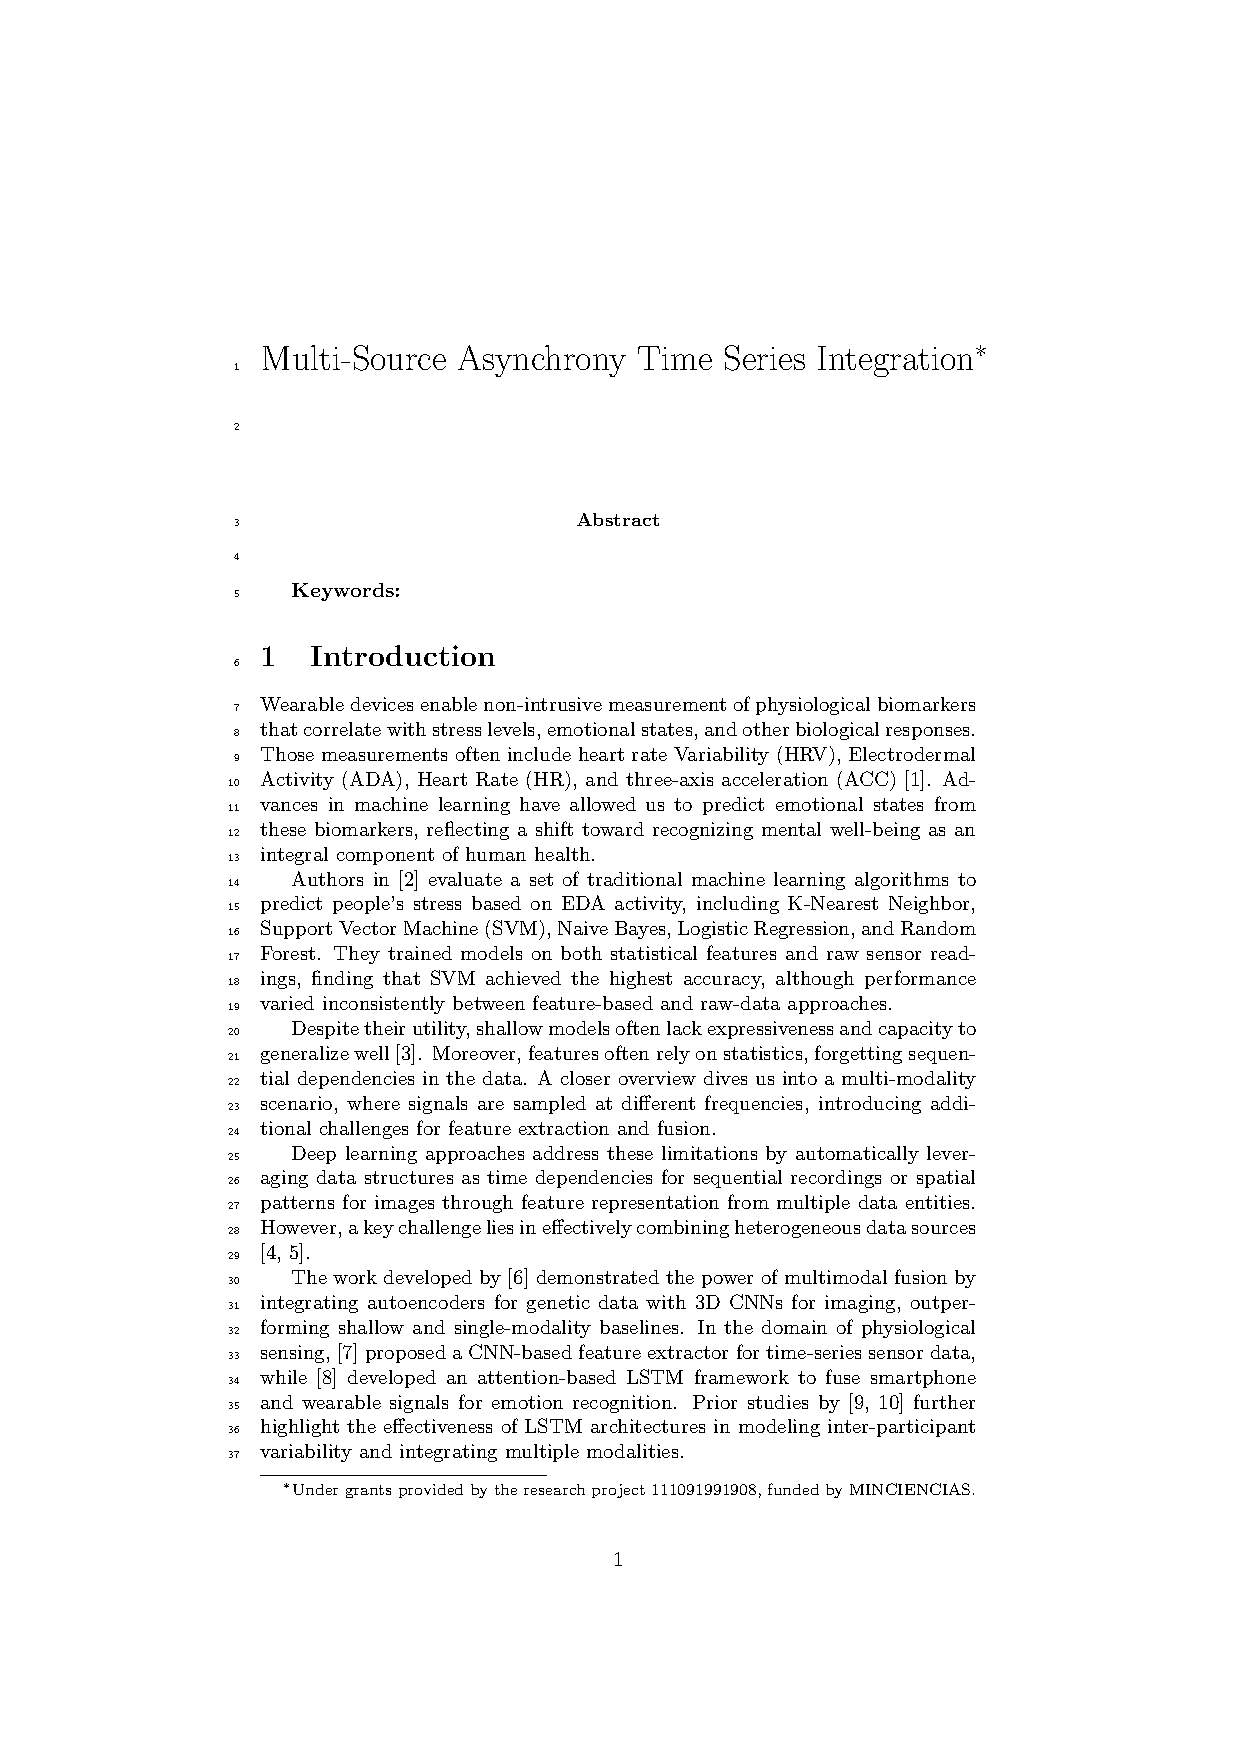
\includepdf[
pages=1,
fitpaper=true,
pagecommand={%
	\thispagestyle{plain}%
	\centering\Large\bfseries Artículo Q1}%
]{../paper_draft/main.pdf}

% Resto del segundo anexo
\includepdf[
pages=2-last,
fitpaper=true,
pagecommand={}
]{../paper_draft/main.pdf}
